\parindent=0em
\section{Shader de oclusión}
\noindent

El \textit{shader} de oclusión es la alternativa al \textit{shader} de profundidad. En este caso, se utiliza la nube de puntos de profundidad para generar una malla de oclusión (explicada en la sección~\ref{sec:oclusion}) y se le aplica dicho \textit{shader} a estas mallas para que actúen de planos que ocluyan los objetos virtuales.\\

El \textit{shader} de oclusión se basa en 3 puntos fundamentales para su funcionamiento:

\begin{itemize}
    \item \textit{ZWrite}:
    \item \textit{ZTest}:
    \item \textit{ColorMask}:
\end{itemize}

Para la prueba de este \textit{shader} en primer lugar se escanea el área para que ARCore genere la nube de puntos y una dichos puntos entre sí para generar planos con distintos ángulos en los que detecta objetos. Para visualizar mejor estas mallas de oclusión se les ha aplicado un contorno negro (figura~\ref{fig:mallaARCoreoclusion}).

\begin{figure}[H]
\centering
    \hspace{-4mm}
    \begin{minipage}{0.5\textwidth}
        \centering
        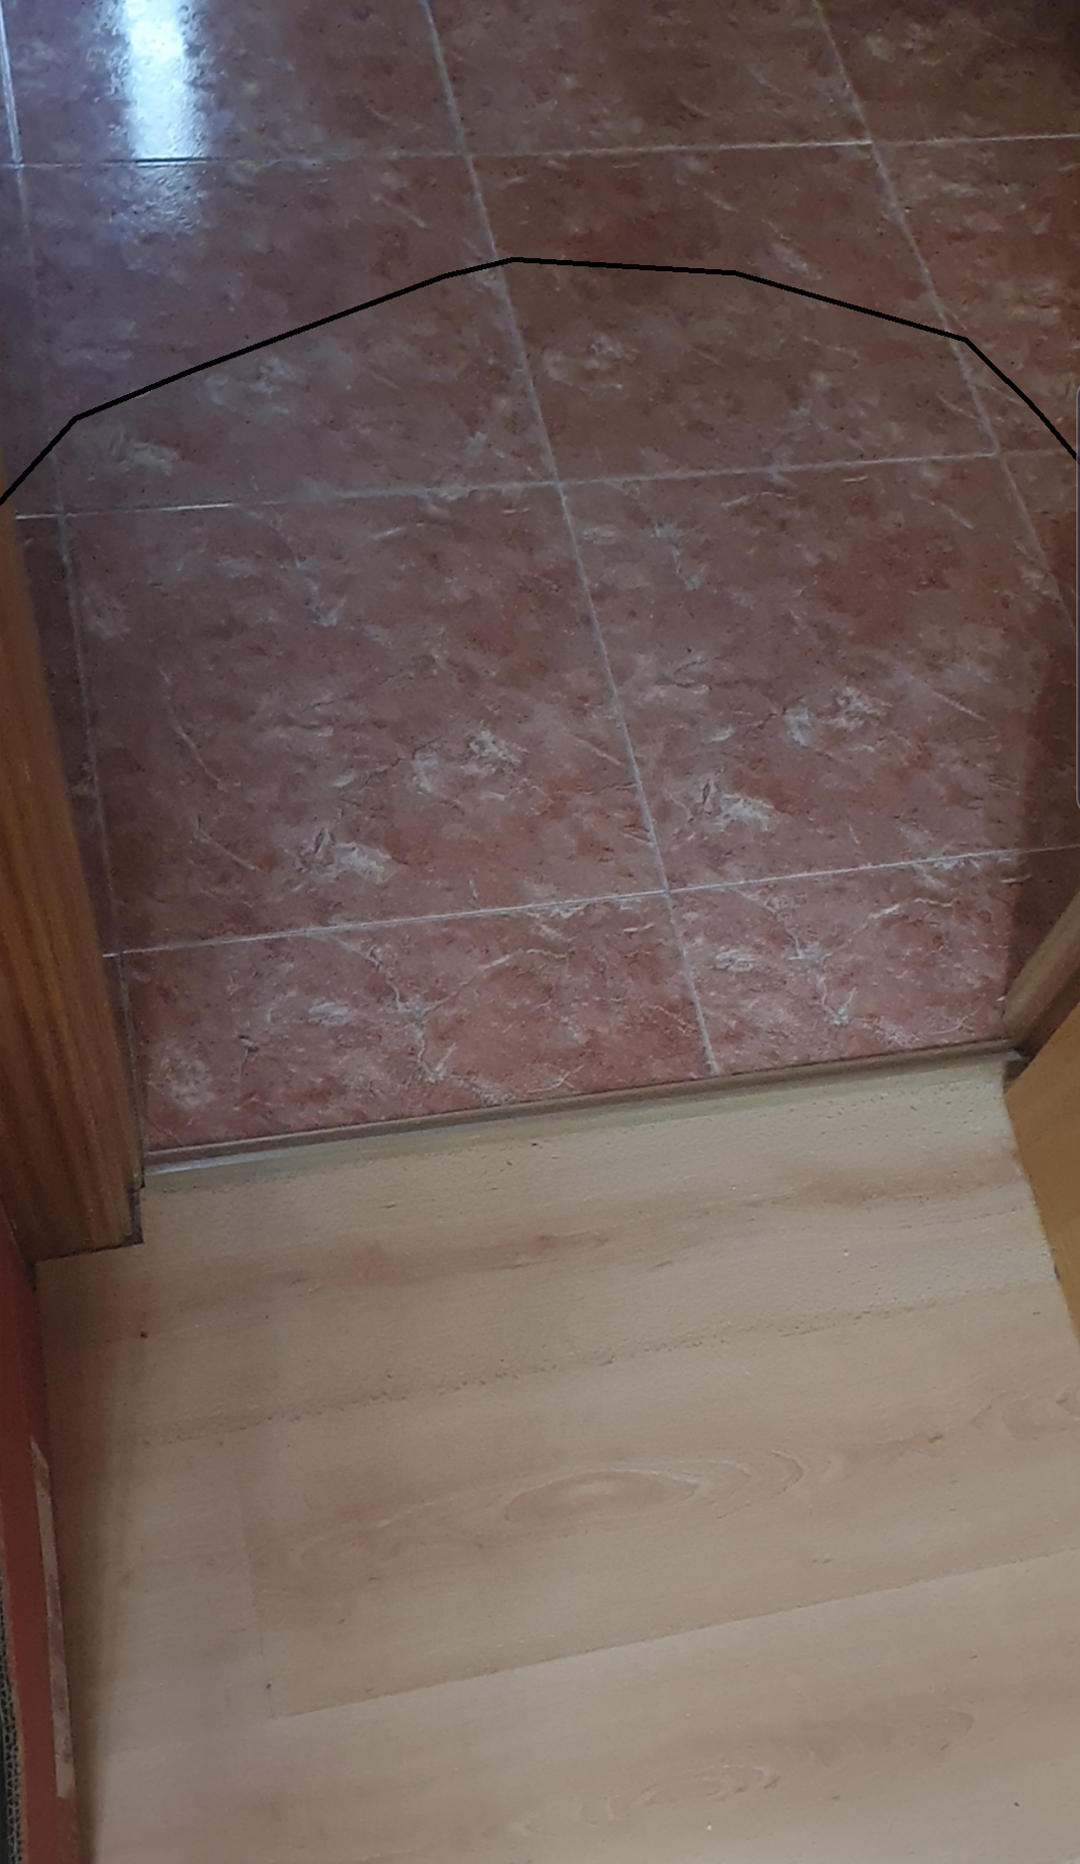
\includegraphics[scale=0.15]{Images/Shaders/oclusion (1).jpg}\\
    \end{minipage}
    \begin{minipage}{0.5\textwidth}
        \centering
        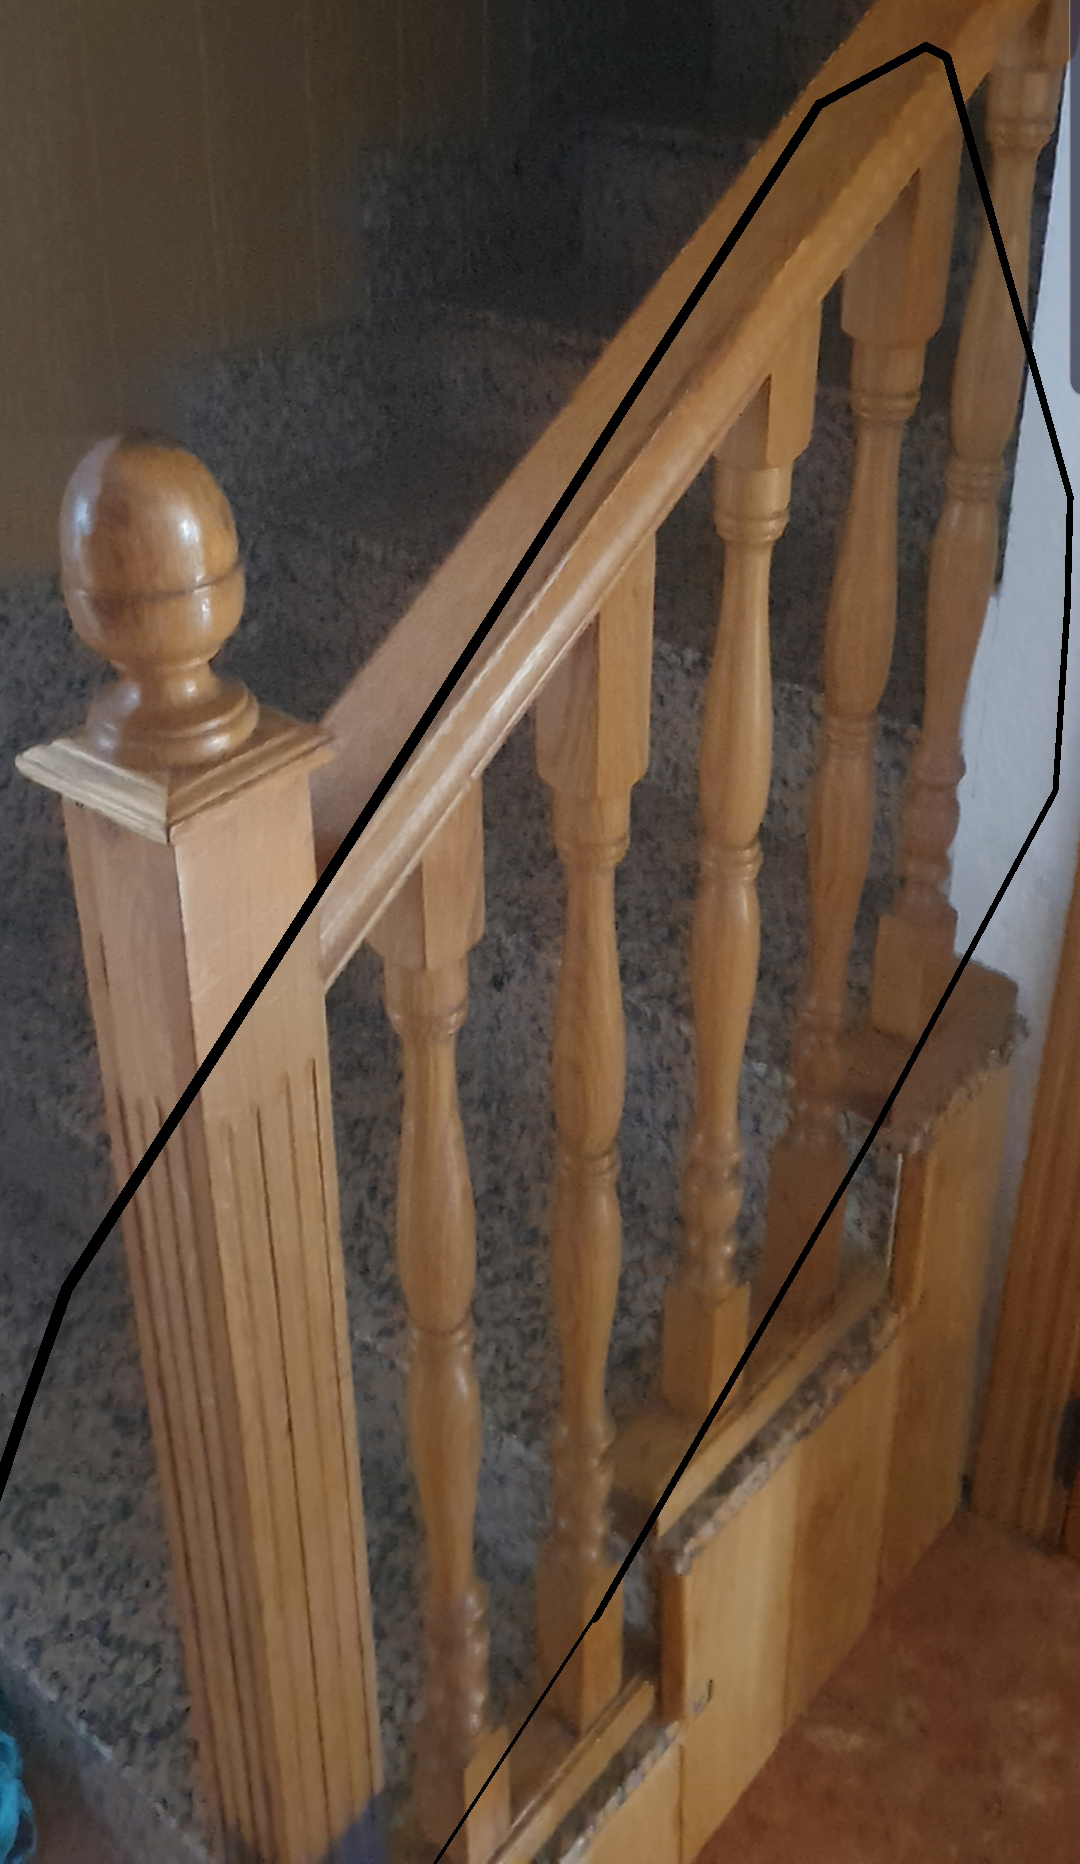
\includegraphics[scale=0.15]{Images/Shaders/oclusion (2).jpg}\\
    \end{minipage}\\
    \caption[Generación de malla de ARCore con contorno]{Generación de malla de ARCore con contorno.}
    \label{fig:mallaARCoreoclusion}
\end{figure}

Es necesario escanear el área varias veces para que ARCore genere todos los planos del área en el que se quiere generar el efecto de oclusión, una vez hecho esto, se coloca un objeto (en este caso un cubo de color rojo) en uno de los planos. En la figura~\ref{fig:oclusionp1} se puede apreciar como el proceso de aplicar el \textit{shader} de oclusión a los planos genera un buen efecto de oclusión. Esto ocurre ya que se coloca el cubo en un plano a la altura del suelo y, por encima de este, existe el plano generado debido a la mesa que hace de malla de oclusión para el elemento virtual. 

\begin{figure}[H]
    \centering
    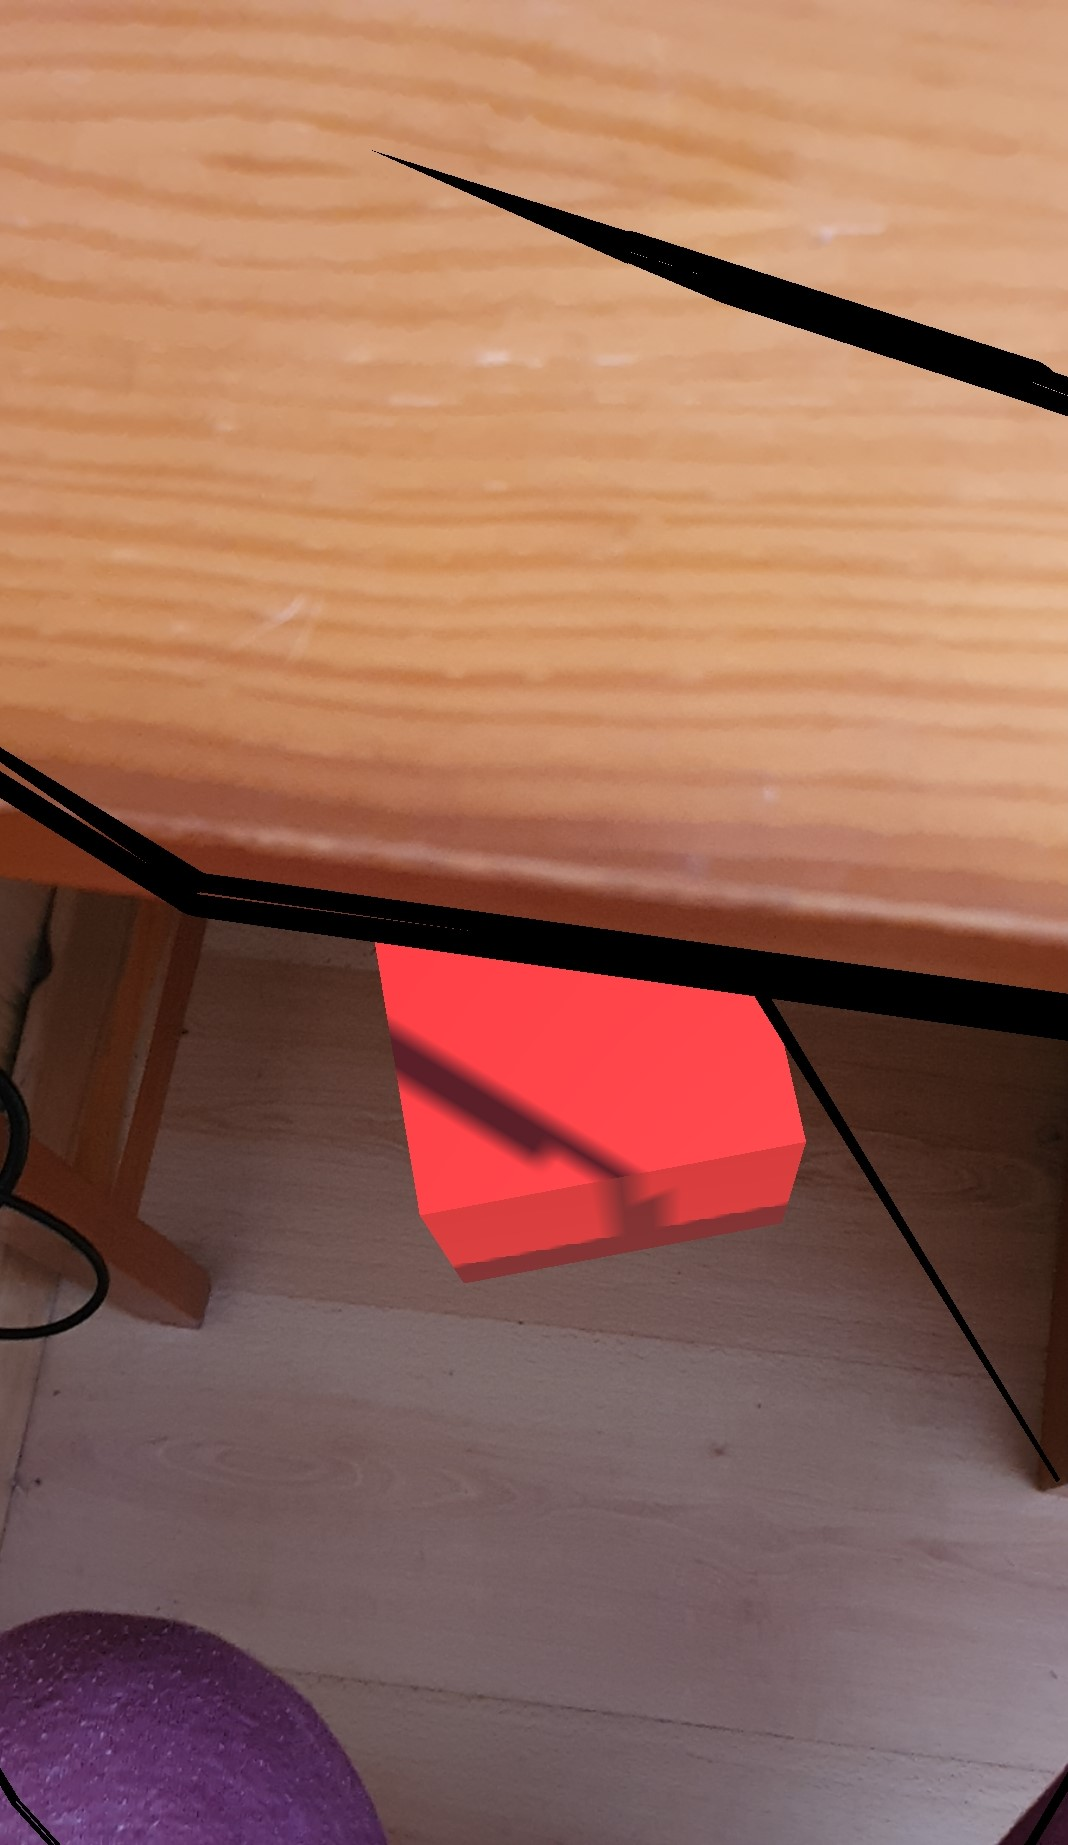
\includegraphics[scale=0.2]{Images/Shaders/oclusionPrueba1.jpg}
    \caption{Efecto de oclusión generado con el \textit{shader} de oclusión.}
    \label{fig:oclusionp1}
\end{figure} 

Después de obtener estos resultados en elementos pequeños y cercanos al dispositivo, se pasó a comprobar la eficacia del \textit{shader} en elementos más grandes y más distantes del dispositivo, ya que el objetivo principal era generar efecto de oclusión en esquinas.\\

Como se puede ver en las pruebas que se realizaron en una esquina y en un objeto grande y detallado como una silla \textit{gaming} (figura~\ref{fig:shaderprofprueba2}), la generación de mallas de ARCore al menos en dispositivos con cámara monocular se ajusta poco a la realidad, es decir, los planos generados no son precisos. Esto provoca que el efecto de oclusión no sea preciso en estos casos en los que los elementos son grandes y distantes al dispositivo o grandes y con geometrías detalladas.

\begin{figure}[H]
\centering
    \hspace{-4mm}
    \begin{minipage}{0.5\textwidth}
        \centering
        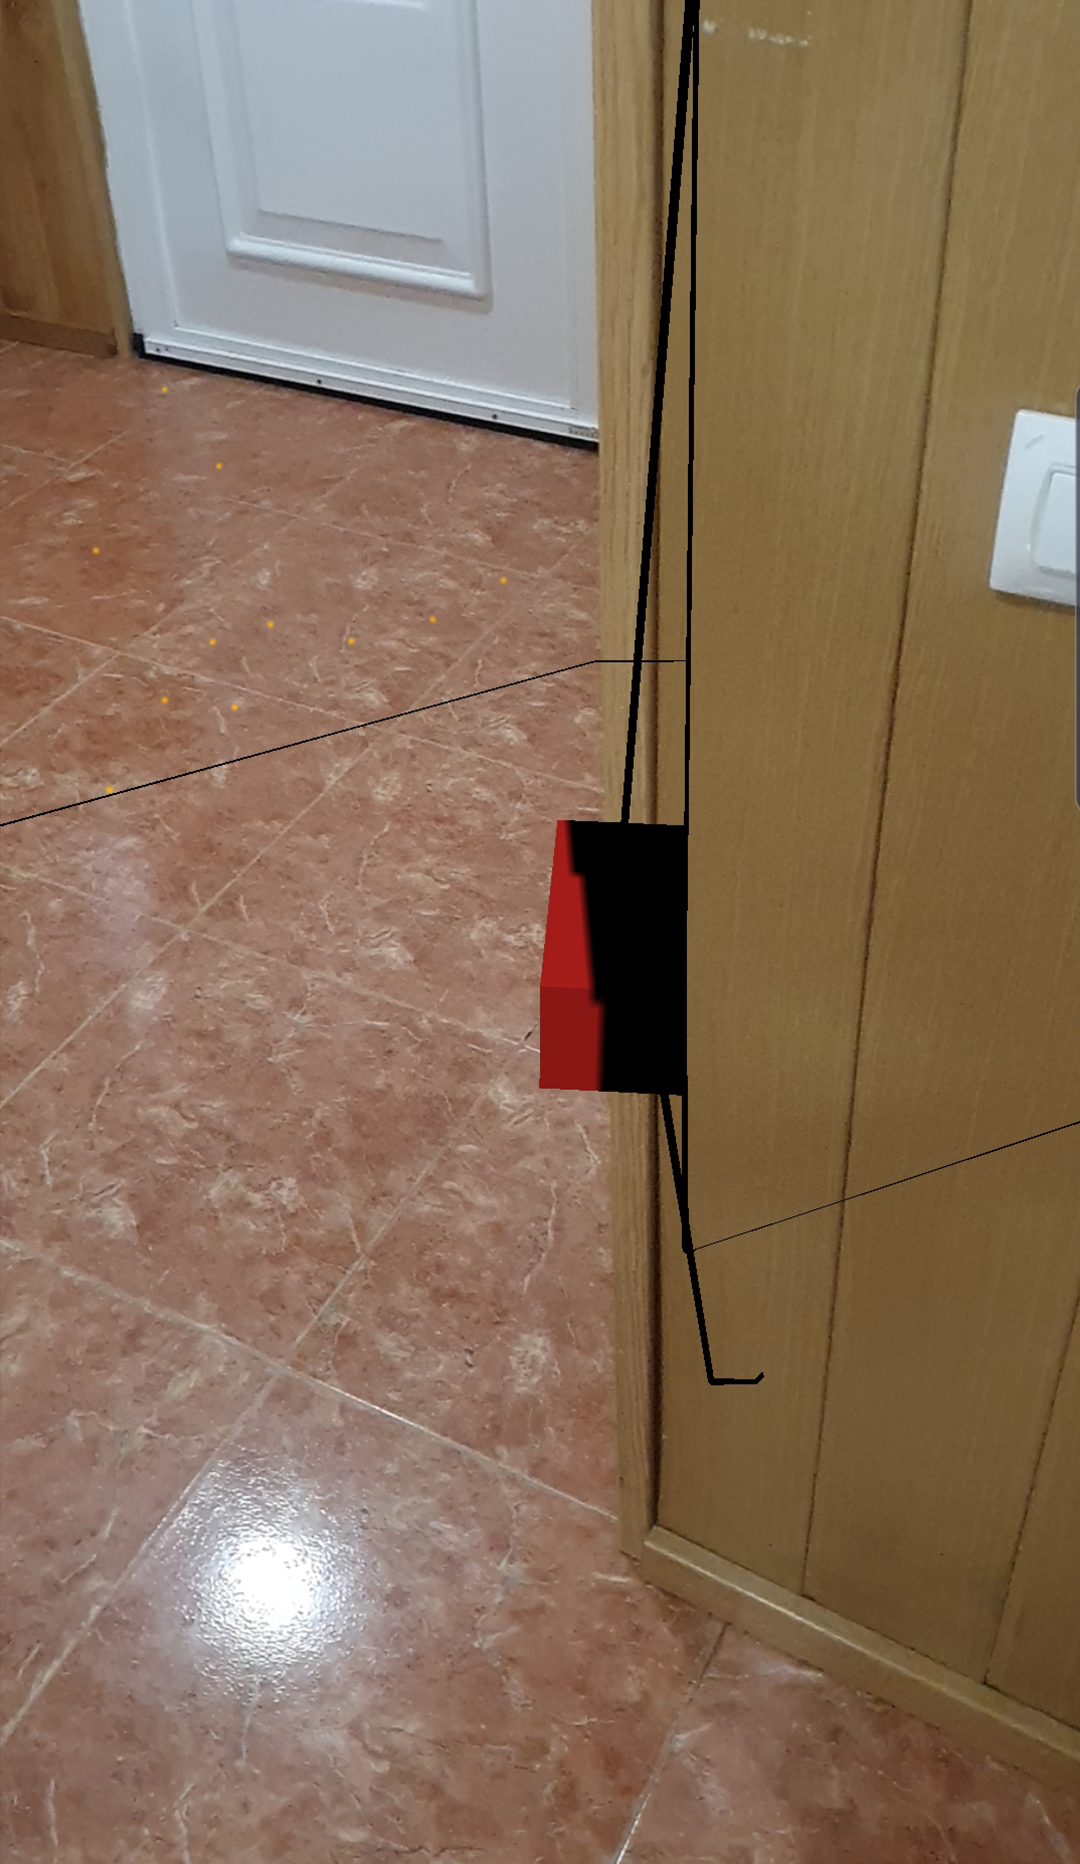
\includegraphics[scale=0.15]{Images/Shaders/oclusionprueba2 (1).jpg}\\
    \end{minipage}
    \begin{minipage}{0.5\textwidth}
        \centering
        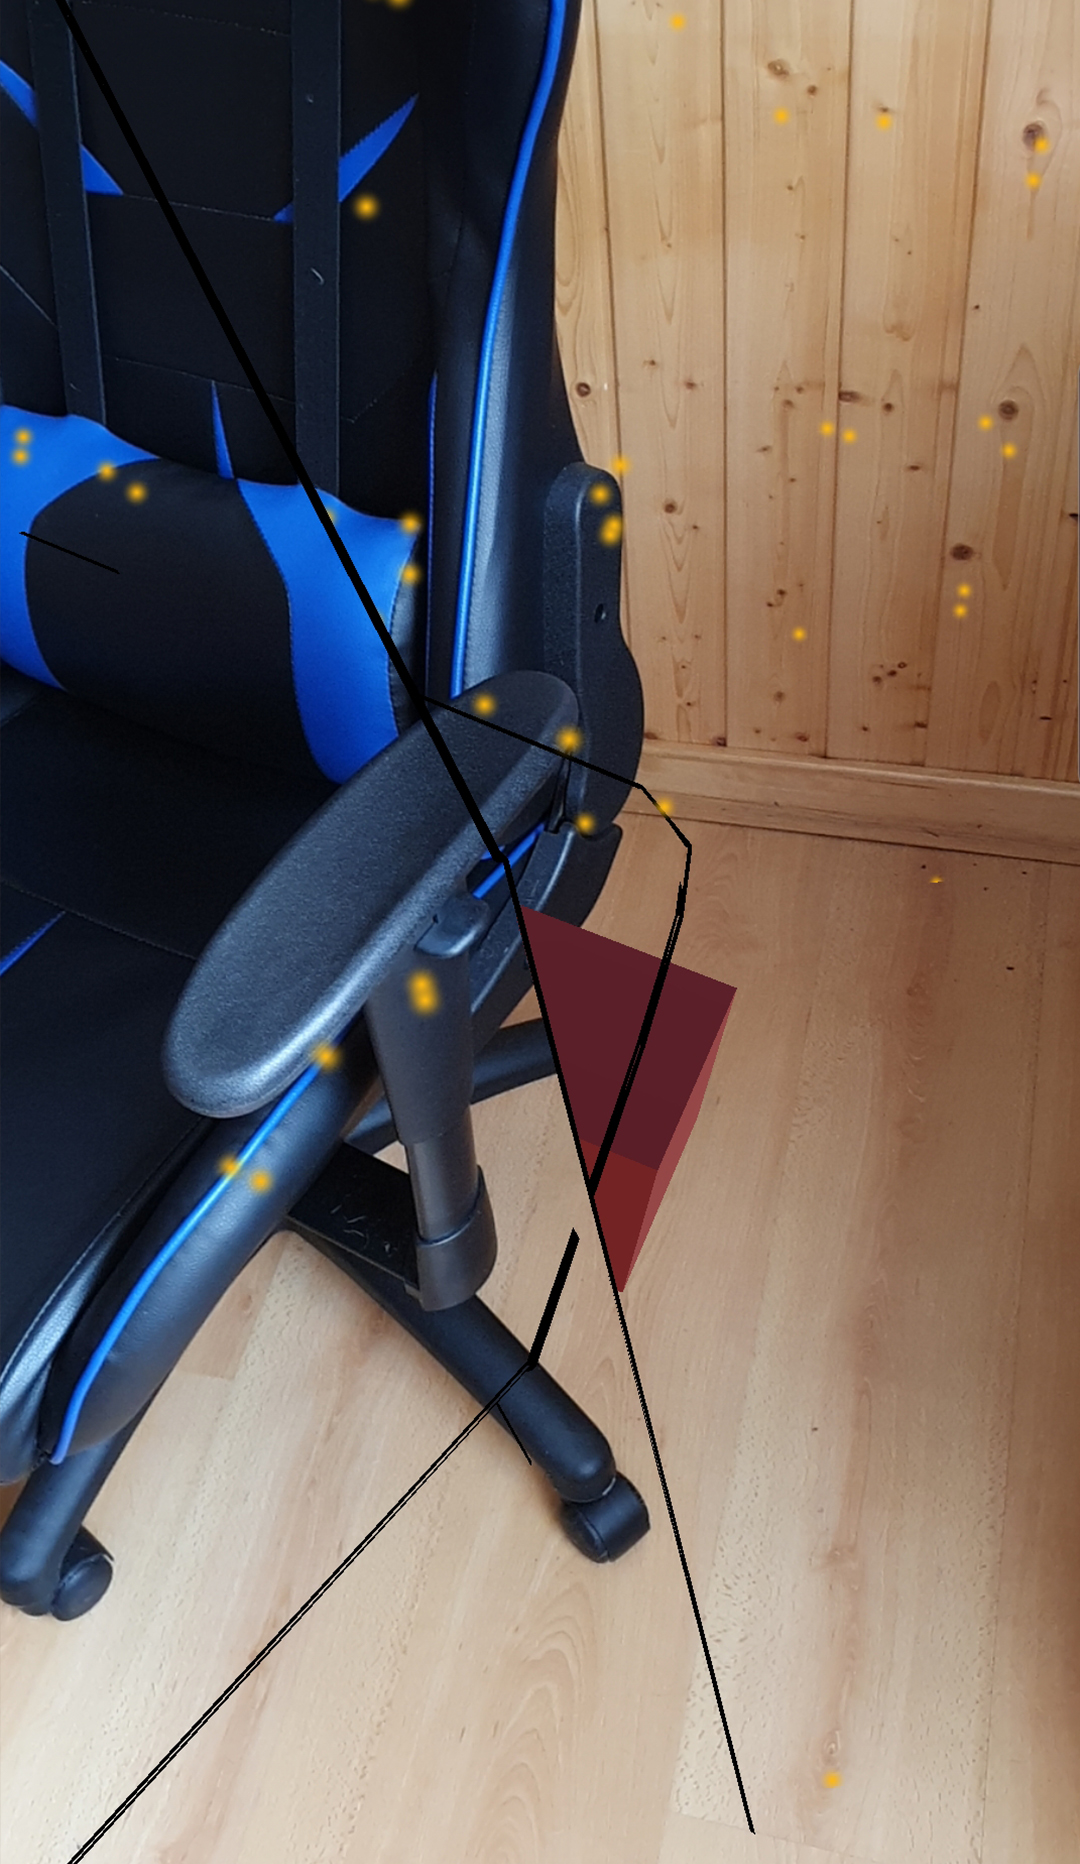
\includegraphics[scale=0.15]{Images/Shaders/oclusionprueba2 (2).jpg}\\
    \end{minipage}\\
    \caption{Pruebas del \textit{shader} de oclusión en esquinas y objetos con geometrías detalladas.}
    \label{fig:shaderprofprueba2}
\end{figure}

Dado que el problema en este caso era que los planos generados por ARCore uniendo la nube de puntos eran imprecisos y el \textit{shader} de oclusión funcionaba correctamente, se pasó a dejar de unir los puntos de la nube para generar planos y hacer una malla de oclusión a simplemente generar la nube y colocar primitivas (que tenía en el \textit{shader} de oclusión aplicado) en dichos puntos para generar el efecto de oclusión. 